%GiG
\documentclass{beamer} 
\usetheme{Copenhagen}
\setbeamertemplate{navigation symbols}{}
\setbeamertemplate{headline}{}
\DeclareMathOperator*{\argmax}{arg\,max}

\usepackage{hyperref}


\definecolor{azure}{rgb}{0.0, 0.5, 1.0}
%\newcommand{\tblue}[1]{\textcolor{blue}{#1}}
\newcommand{\tblue}[1]{{\Large {\textcolor{azure}{#1}}}}
\newcommand{\thblue}[1]{{\Huge {\textcolor{azure}{#1}}}}
\newcommand{\hred}[1]{{\textcolor{red}{#1}}}
\newcommand{\furl}[1]{{\footnote{\url{#1}}}}

\title[Saravanan Thirumuruganathan] 
{Lecture 1: Course Introduction and Logistics}

\author[CSE 5334] 
{Instructor: Saravanan Thirumuruganathan}

\date[] 

\begin{document}

\begin{frame}
  \titlepage
\end{frame}

%\begin{frame}{Outline}
%  \tableofcontents
%  % You might wish to add the option [pausesections]
%\end{frame}

\section{Outline}

\begin{frame}
\frametitle {Outline}
\begin{enumerate}
\item Data Mining/Science Basics
\item Logistics
\item Scientific Python
\item IPython Notebook Demo
\end{enumerate}
\end{frame}

%\begin{frame}{In-Class Quizzes}
%\begin{itemize}
%\item {\Large {\bf URL:}} {\LARGE \bf \url{http://m.socrative.com/}} 
%\item {\Large {\bf Room Name:} {\LARGE \bf 4f2bb99e}}
%\end{itemize}
%\end{frame}

\section{Data Mining Introduction}
\begin{frame}{}
    \begin{center}
        \thblue{Introduction To Data Mining/Science}
    \end{center}
\end{frame}

\begin{frame}{Big Data\footnote{\url{https://www.pinterest.com/pin/101753272804937744/}}}
    \begin{center}
        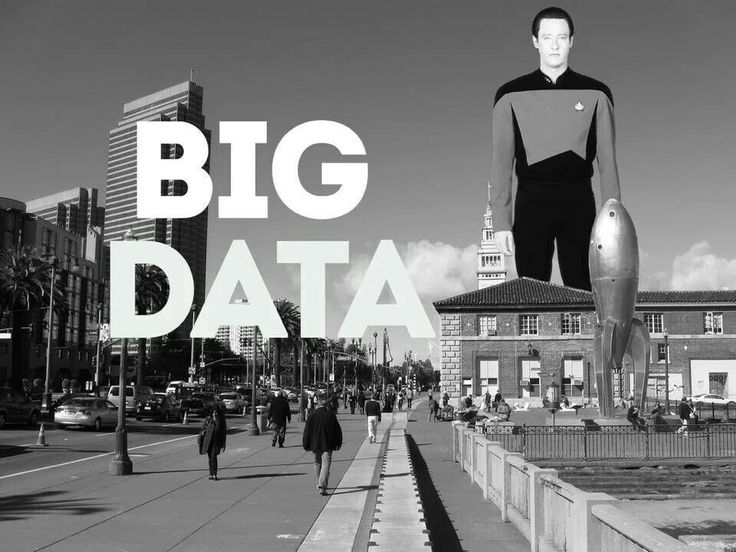
\includegraphics[scale=0.38]{bigDataStarTrek.jpg}
    \end{center}
\end{frame}

\begin{frame}{Big Data\footnote{\url{http://memegenerator.net/instance/55214797}}}
    \begin{center}
        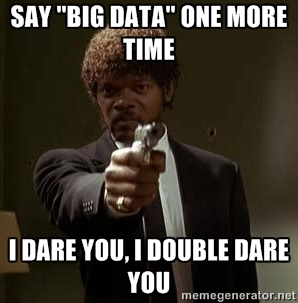
\includegraphics[scale=0.8]{bigDataPulpFiction.jpg}
    \end{center}
\end{frame}

\begin{frame}{Big Data}
    \begin{center}
        {\Large``Between the dawn of civilization and 2003, we only created five exabytes of information; now we're creating that amount every two days.'' \\ 
        ~\\ \qquad \qquad - Eric Schmidt, Google} \\ 
        ~\\~\\
        One Second on the Internet: \url{http://onesecond.designly.com/}
    \end{center}
\end{frame}

\begin{frame}{Smarter Devices}
    \begin{center}
        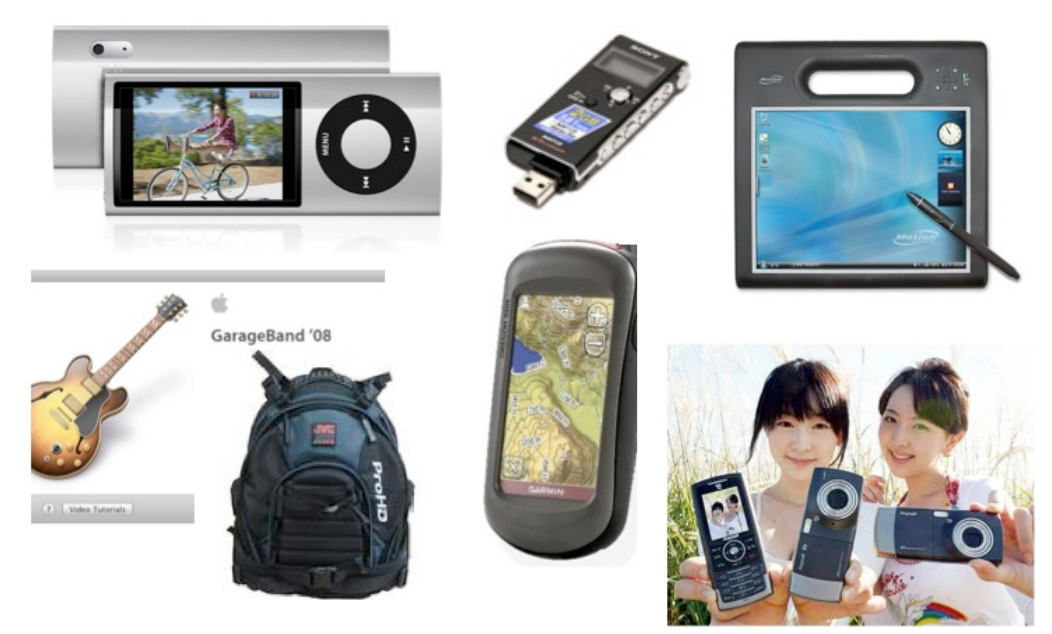
\includegraphics[scale=0.28]{smarterDevices.png}
    \end{center}
\end{frame}
\begin{frame}{Commodity Computing}
    \begin{center}
        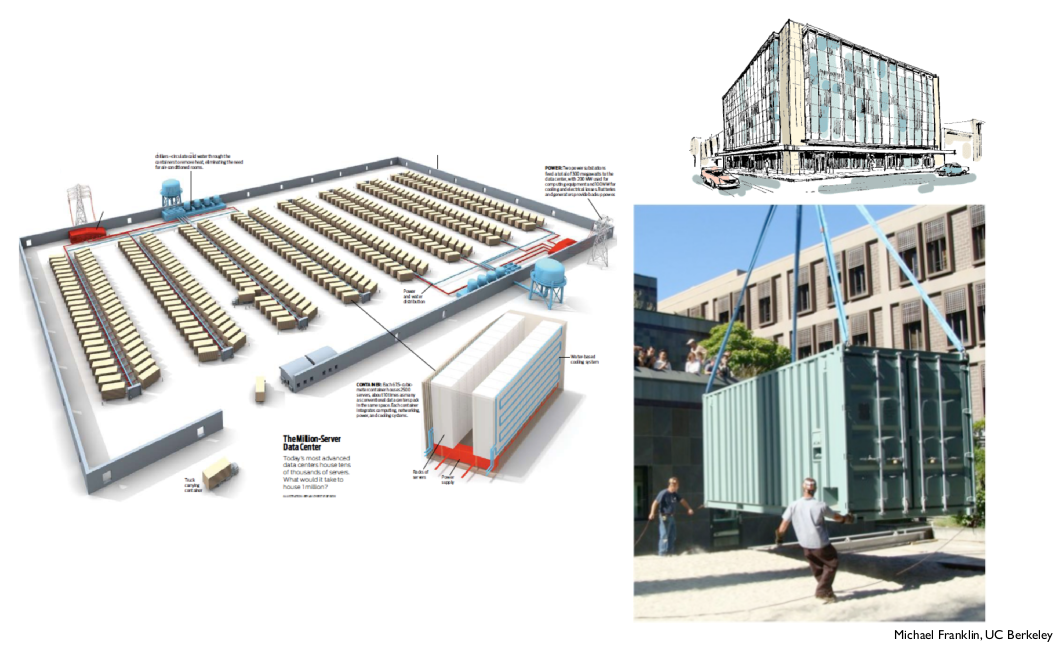
\includegraphics[scale=0.28]{commodityComputing.png}
    \end{center}
\end{frame}
\begin{frame}{Ubiquitous Connectivity}
    \begin{center}
        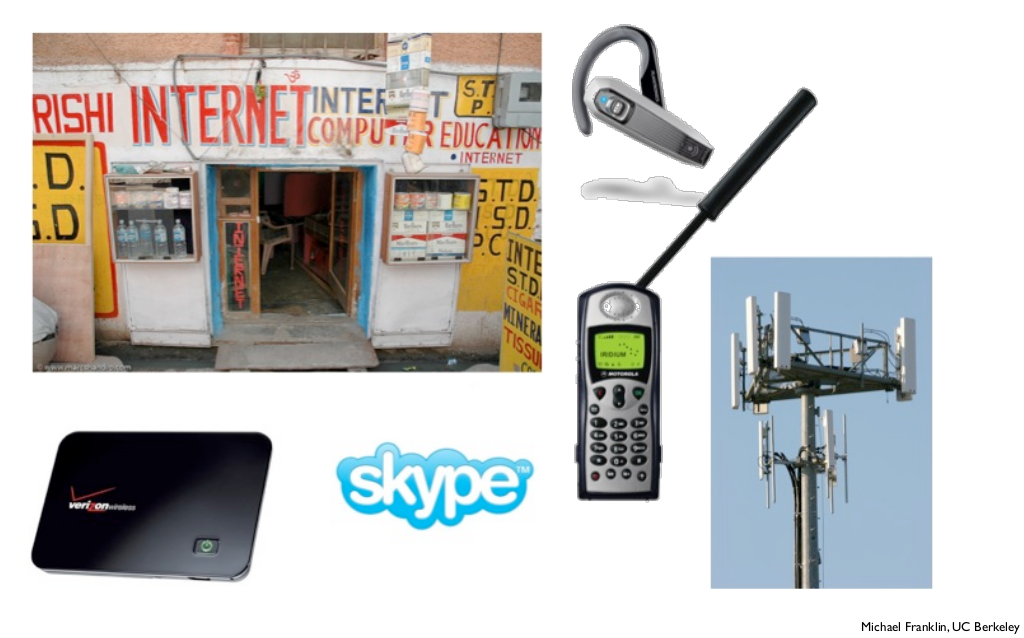
\includegraphics[scale=0.28]{ubiquitousConnectivity.png}
    \end{center}
\end{frame}

\begin{frame}{Big Data - 4 V's}
    \begin{itemize}
        \item Volume
        \item Velocity
        \item Variety
        \item {\em Veracity}
    \end{itemize}
\end{frame}


\begin{frame}{}
    \begin{center}
        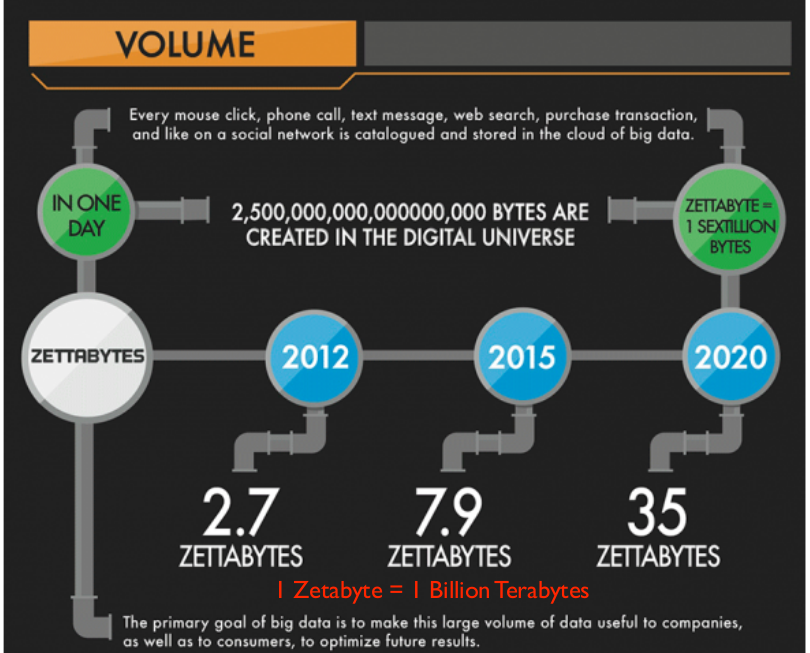
\includegraphics[scale=0.34]{bigDataVolume.png}
    \end{center}
\end{frame}
\begin{frame}{}
    \begin{center}
        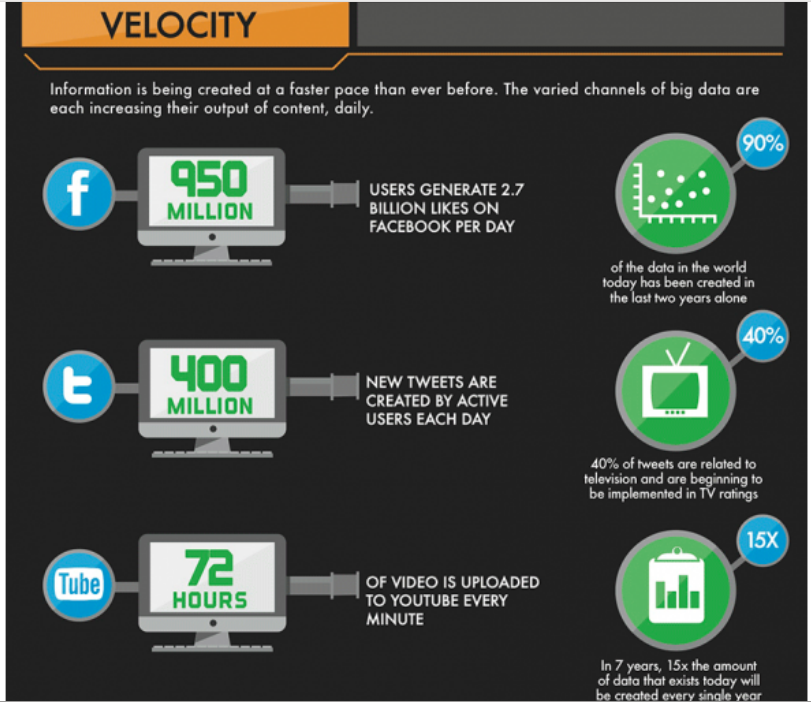
\includegraphics[scale=0.34]{bigDataVelocity.png}
    \end{center}
\end{frame}
\begin{frame}{}
    \begin{center}
        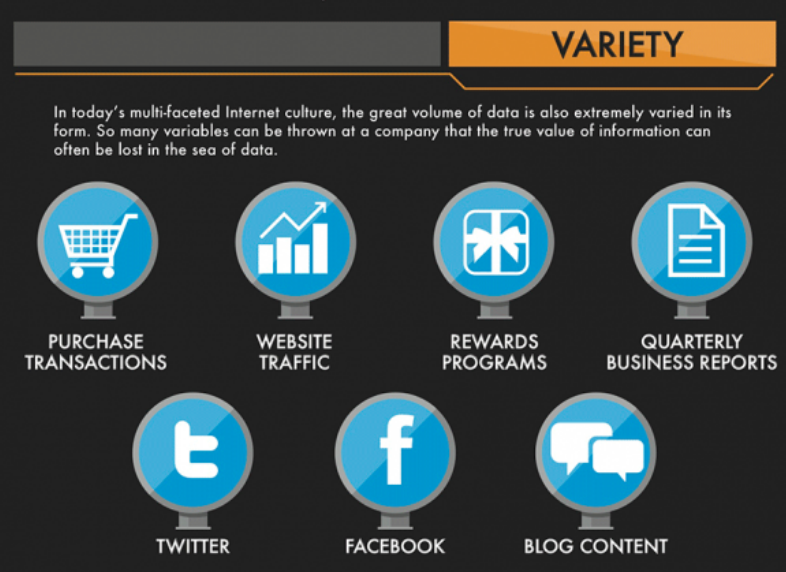
\includegraphics[scale=0.4]{bigDataVariety.png}
    \end{center}
\end{frame}
\begin{frame}{}
    \begin{center}
        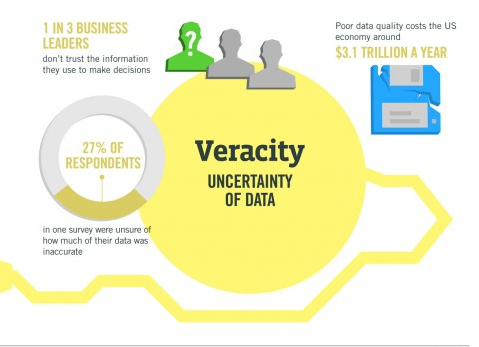
\includegraphics[scale=0.5]{bigDataVeracity.png}\footnote{\url{http://www.ibmbigdatahub.com/}}
    \end{center}
\end{frame}


\begin{frame}{}
    \begin{center}
        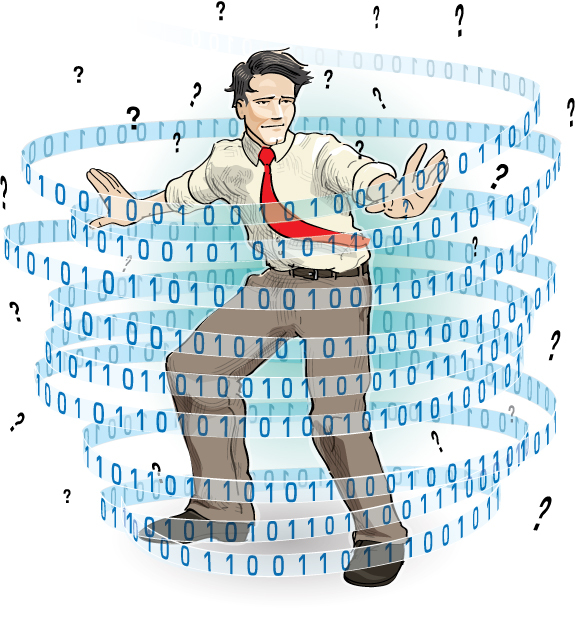
\includegraphics[scale=0.5]{dataHero.jpg}\footnote{\url{https://www.behance.net/gallery/5958295/Data-Hero-Oya-Group}}
    \end{center}
\end{frame}

\begin{frame}{Data Mining}
    \begin{itemize}
        \item Process of semi‐automatically analyzing large databases to find {\bf patterns} that are 
        \begin{itemize}
            \item {\bf valid}: hold on new data with some certainty
            \item {\bf novel}: non‐obvious to the system
            \item {\bf useful}: should  be possible to act on the item
            \item {\bf understandable}: humans should be able to interpret the pattern
        \end{itemize}
    \end{itemize}
\end{frame}
\begin{frame}{}
    \begin{center}
        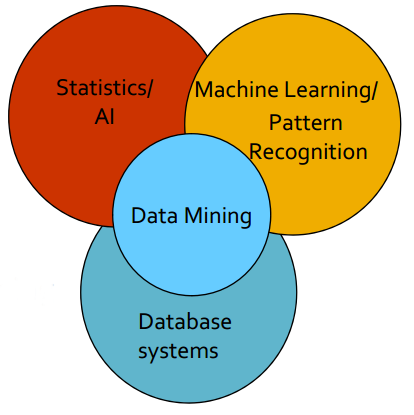
\includegraphics[scale=0.5]{dataMiningVennDiagram.png}
    \end{center}
\end{frame}

\begin{frame}{Data Science}
    \begin{itemize}
       \item To gain insights into data through computation, statistics, and visualization
       \item ``A data scientist is someone who knows more statistics than a computer scientist and more computer science than a statistician'' - Josh Blumenstock
    \end{itemize}
\end{frame}
\begin{frame}{}
    \begin{center}
        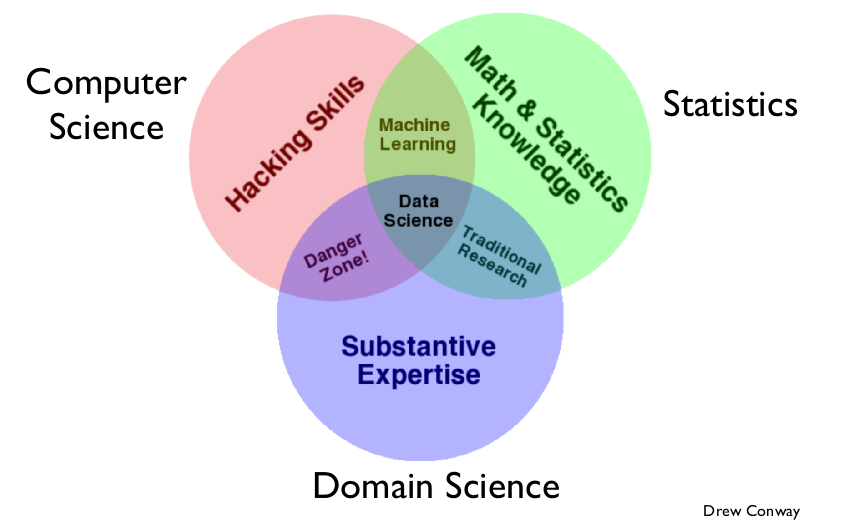
\includegraphics[scale=0.4]{dataScienceVennDiagram.png}
    \end{center}
\end{frame}


\begin{frame}{Google}
    \begin{center}
        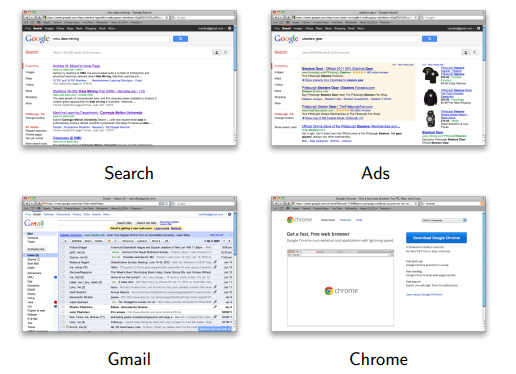
\includegraphics[scale=0.5]{google.png}
    \end{center}
\end{frame}
\begin{frame}{Facebook}
    \begin{center}
        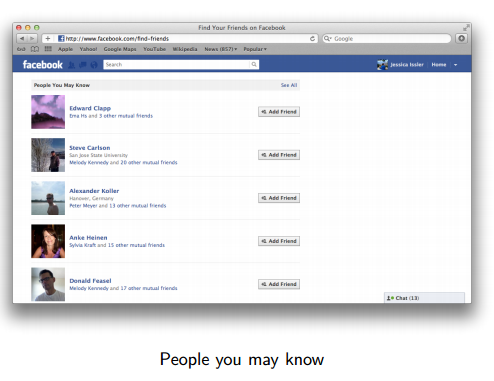
\includegraphics[scale=0.5]{facebook.png}
    \end{center}
\end{frame}
\begin{frame}{Netflix}
    \begin{center}
        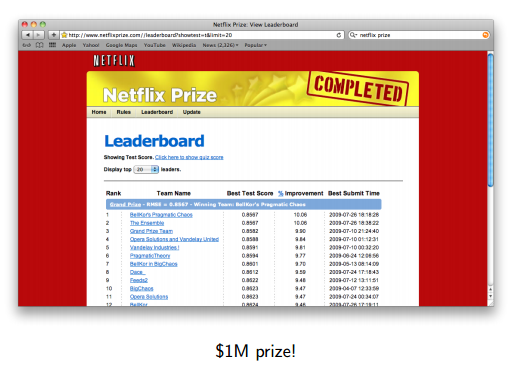
\includegraphics[scale=0.5]{netflix.png}
    \end{center}
\end{frame}
\begin{frame}{eHarmony}
    \begin{center}
        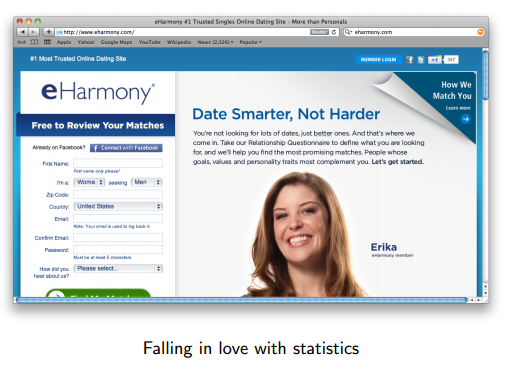
\includegraphics[scale=0.5]{eHarmony.png}
    \end{center}
\end{frame}
\begin{frame}{FICO}
    \begin{center}
        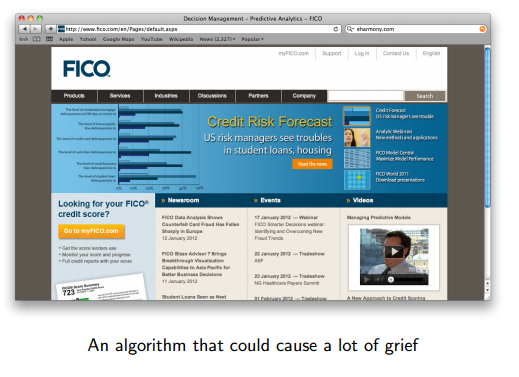
\includegraphics[scale=0.5]{fico.png}
    \end{center}
\end{frame}
\begin{frame}{FlightCaster}
    \begin{center}
        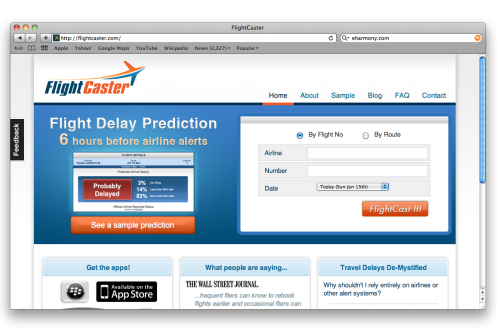
\includegraphics[scale=0.5]{flightCaster.png}
    \end{center}
\end{frame}
\begin{frame}{IBM's Watson}
    \begin{center}
        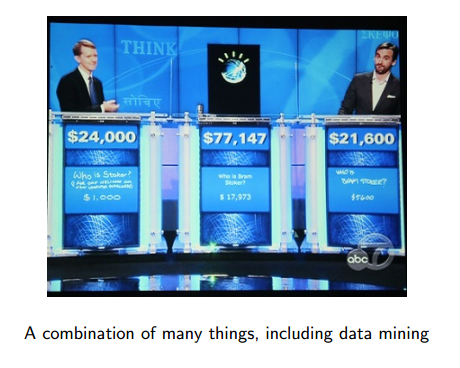
\includegraphics[scale=0.5]{watson.png}
    \end{center}
\end{frame}
\begin{frame}{Handwritten postal codes}
    \begin{center}
        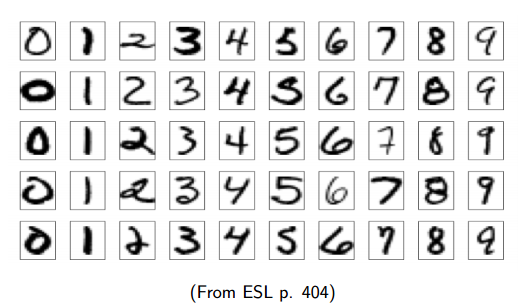
\includegraphics[scale=0.5]{ocr.png}
    \end{center}
\end{frame}

\begin{frame}
    \begin{center}
        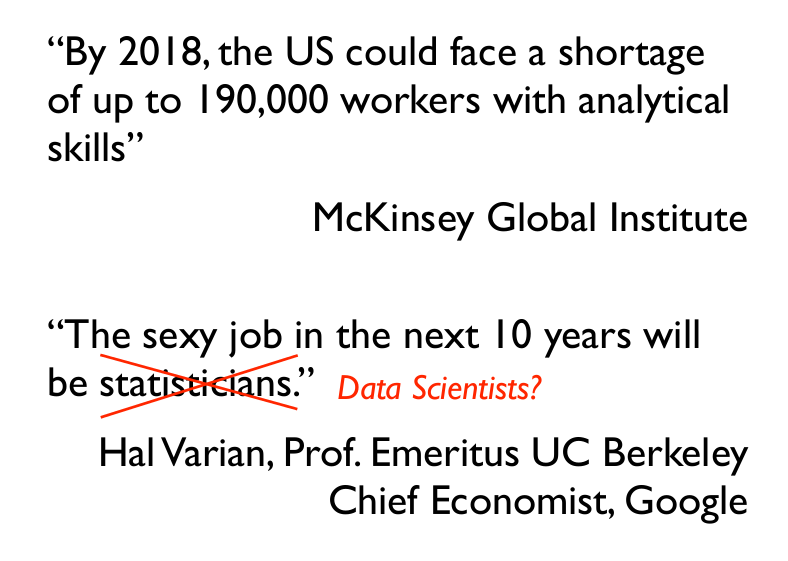
\includegraphics[scale=0.3]{dmJobs.png}
    \end{center}
\end{frame}


\section{Logistics}

\begin{frame}{}
    \begin{center}
        \thblue{Logistics}
    \end{center}
\end{frame}

\begin{frame}{My Background}
    \begin{itemize}
        \item Saravanan Thirumuruganathan
        \item Final year PhD Student working with Dr.Gautam Das
        \item Website: \url{http://saravananthirumuruganathan.appspot.com}
        \item Interests: Data Mining, Algorithms, Data Exploration, Social Networks, Machine Learning, Artificial Intelligence
    \end{itemize}
\end{frame}

\begin{frame}{Course Details}
    \begin{itemize}
        \item Lectures: TuTh 2-3:30pm, PKH 321
        \item Course Website: \url{http://saravanan-thirumuruganathan.github.io/cse5334Spring2015/index.html}
        \item Instructor: Saravanan Thirumuruganathan
        \begin{itemize}
            \item Mail: firstname.lastname[at]mavs.uta.edu
            \item Office Hours: TuTh 12:30-2:00pm, Fri: 2-5pm or by appointment 
        \end{itemize}
        \item TA: TBD
    \end{itemize}
\end{frame}


\begin{frame}{Piazza}
    \begin{itemize}
        \item Q\&A Platform
        \item ``mixture between a wiki and a forum''
        \item \url{https://piazza.com/class/i551721xpki6w7}
        \item Please use it as much as possible for public/common questions and clarifications
    \end{itemize}
\end{frame}

\begin{frame}{Text Books\footnote{\url{http://www.santabanta.com/}}}
    \begin{center}
        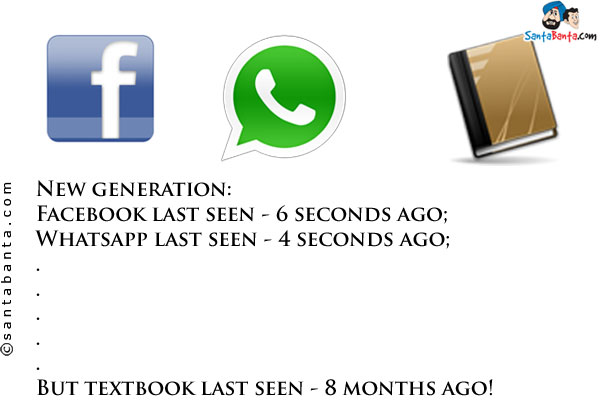
\includegraphics[scale=0.5]{santaBanta.jpg}
    \end{center}
\end{frame}

\begin{frame}{Text Books}
    \begin{itemize}
        \item There is no book to cover them all 
        \item Multiple books (free eBook links in Website)
        \begin{itemize}
            \item {\bf [MMDS]} Mining of Massive Datasets by Jure Leskovec, Anand Rajaraman, Jeff Ullman.
            \item {\bf [DMA]} Data Mining and Analysis: Fundamental Concepts and Algorithms by Mohammed Zaki and Wagner Meira.
            \item {\bf [ISLR]} An Introduction to Statistical Learning with Applications in R. 
            \item {\bf [IIR]} Introduction to Information Retrieval by Christopher D. Manning, Prabhakar Raghavan and Hinrich Schutze.
        \end{itemize}
    \end{itemize}
\end{frame}


\begin{frame}{Grading}
    \begin{itemize}
        \item $5$ Programming Projects: 30\%
        \item Capstone Project: 10\%
        \item Midterm: 30\%
        \item Final : 30\% (non comprehensive)
        \item Grading will be on a curve
    \end{itemize}
\end{frame}


\begin{frame}{Programming Projects}
    \begin{itemize}
        \item Team based, 1-3 members
        \item Coding will be in Python
        \item Some of them will be intensive
        \item Startup code, testing code will be provided
        \item Capstone project
        \item Data Science portfolios
    \end{itemize}
\end{frame}


\begin{frame}{Programming Projects}
    \begin{itemize}
        \item Project/Dataset suggestions welcome!
        \begin{enumerate}
           \item Exploratory Data Analysis using Python, Pandas, Matplotlib and Seaborn.
           \item Classification Algorithms using Scikit-learn 
           \item Clustering using Scikit-learn 
           \item Search Engine Basics 
           \item Recommender Systems using Scipy 
           \item Capstone Project: Putting it all together 
        \end{enumerate}
    \end{itemize}
\end{frame}


\begin{frame}{Late Days}
    \begin{itemize}
        \item Due at $11:59$pm 
        \item $5$ late days per student for the semester
        \item No more than $2$ could be used per project
        \item No increments
        \item Late Penalty: $50$\% per day
        \item No point in submitting after 4 days
    \end{itemize}
\end{frame}


\begin{frame}{Assignment Advice}
    \begin{itemize}
        \item Start early
        \item Find good team members (Piazza support will be provided)
        \item First assignment will be out in $2$ weeks
        \item Okay to change teams per project
        \item Everyone in team gets same score
        \item Collaboration/Brainstorming is Okay!
        \item No plagiarism!
    \end{itemize}
\end{frame}


\begin{frame}{Data Science Process}
    \begin{center}
        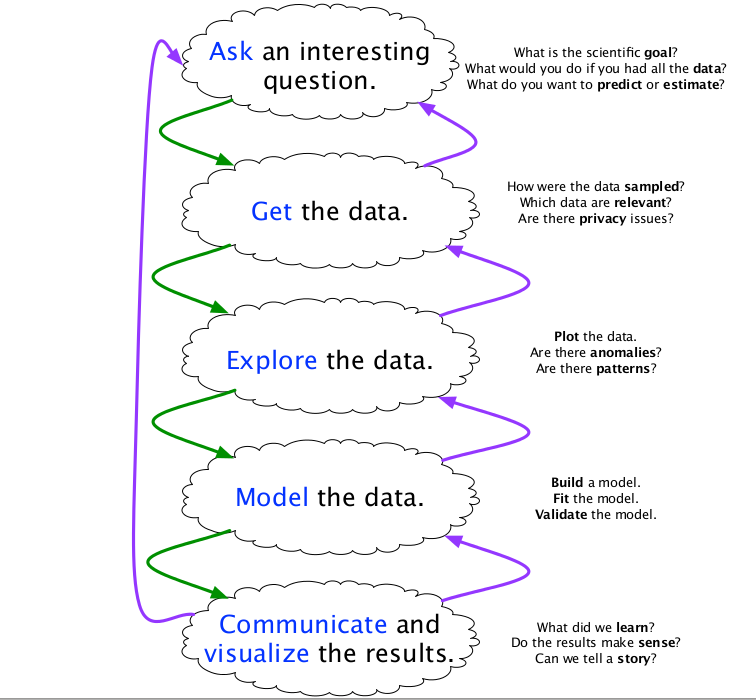
\includegraphics[scale=0.32]{dataScienceProcess.png}
    \end{center}
\end{frame}
\begin{frame}{Topics Covered}
    \begin{itemize}
        \item Data collection, visualization
        \item Exploratory data analysis
        \item Classifiers and Ensembles
        \item Clustering
        \item Search engine basics
        \item Recommender basics
        \item Lot of useful tools: dimensionality reduction, feature selection, hypothesis testing, sampling etc
    \end{itemize}
\end{frame}


\begin{frame}{}
    \begin{center}
        \thblue{Scientific Python}
    \end{center}
\end{frame}

\begin{frame}{}
    \begin{center}
        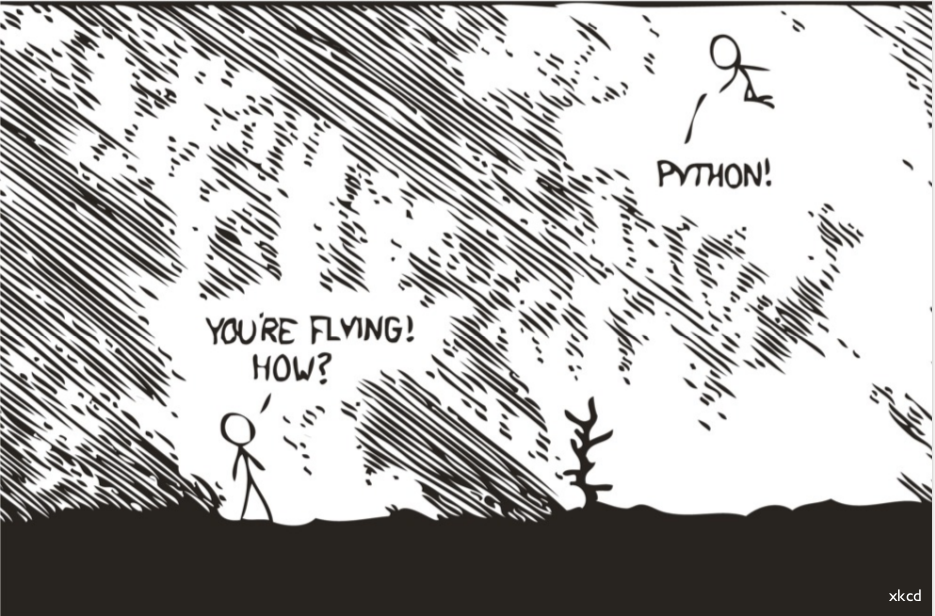
\includegraphics[scale=0.3]{python.png}
    \end{center}
\end{frame}
\begin{frame}{}
    \begin{center}
        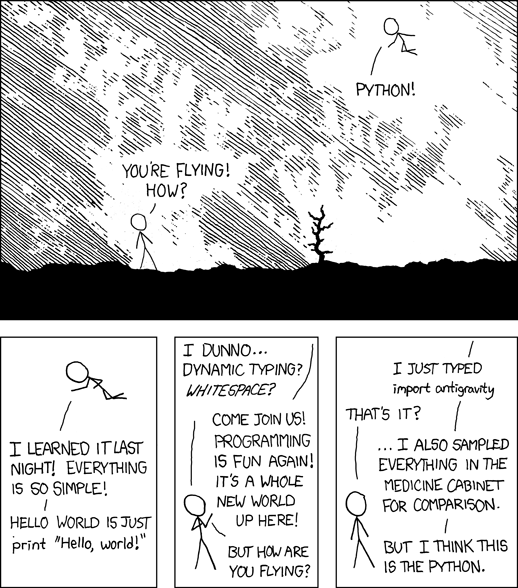
\includegraphics[scale=0.35]{python2.png}
    \end{center}
\end{frame}
\begin{frame}{}
    \begin{center}
        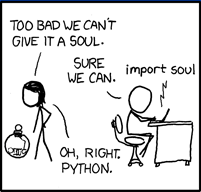
\includegraphics[scale=0.7]{python4.png}
    \end{center}
\end{frame}
\begin{frame}{}
    \begin{center}
        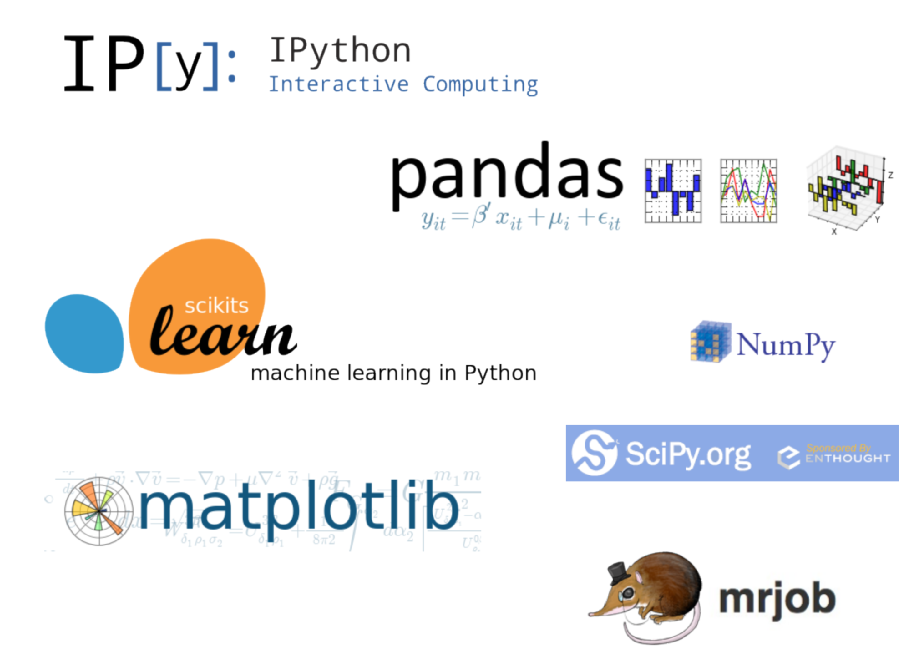
\includegraphics[scale=0.3]{scientificPython.png}
    \end{center}
\end{frame}

\begin{frame}{}
    \begin{center}
        \thblue{IPython Notebooks}
    \end{center}
\end{frame}
\begin{frame}{Process Books}
    \begin{center}
        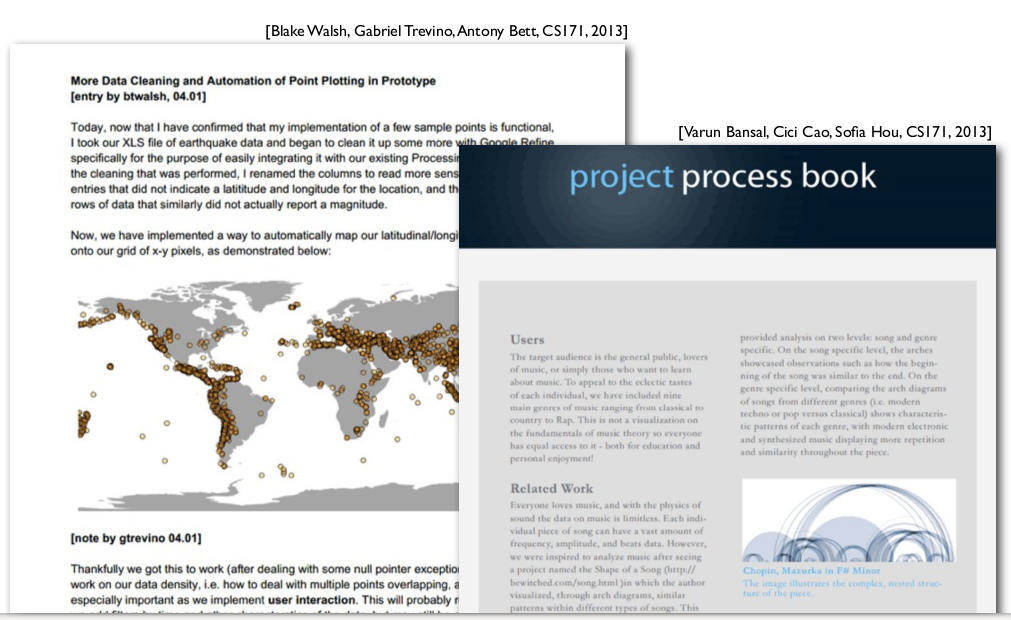
\includegraphics[scale=0.3]{processBooks.png}
    \end{center}
\end{frame}
\begin{frame}{IPython Notebooks}
    \begin{center}
        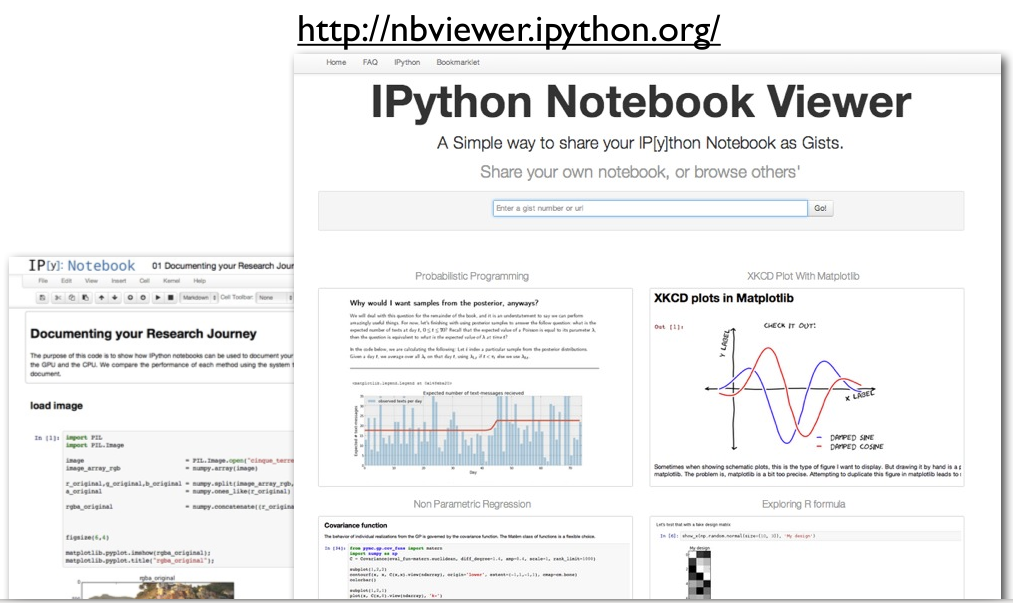
\includegraphics[scale=0.3]{ipythonNotebooks.png}
    \end{center}
\end{frame}
\begin{frame}{}
    \begin{center}
        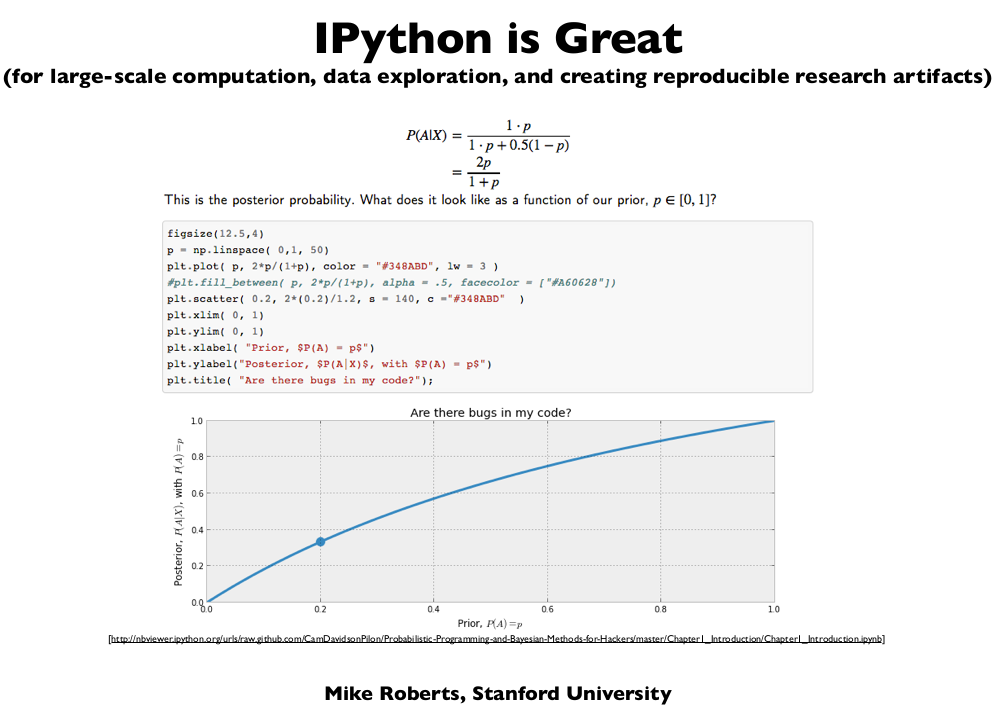
\includegraphics[scale=0.3]{ipythonIsGreat.png}
    \end{center}
\end{frame}
\begin{frame}{}
    \begin{center}
        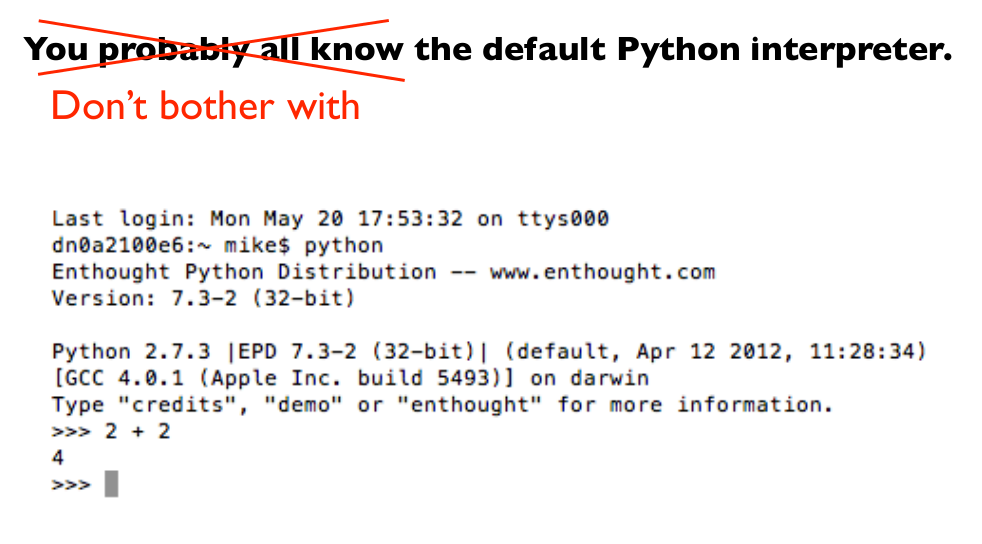
\includegraphics[scale=0.3]{pythonInterpreter.png}
    \end{center}
\end{frame}
\begin{frame}{}
    \begin{center}
        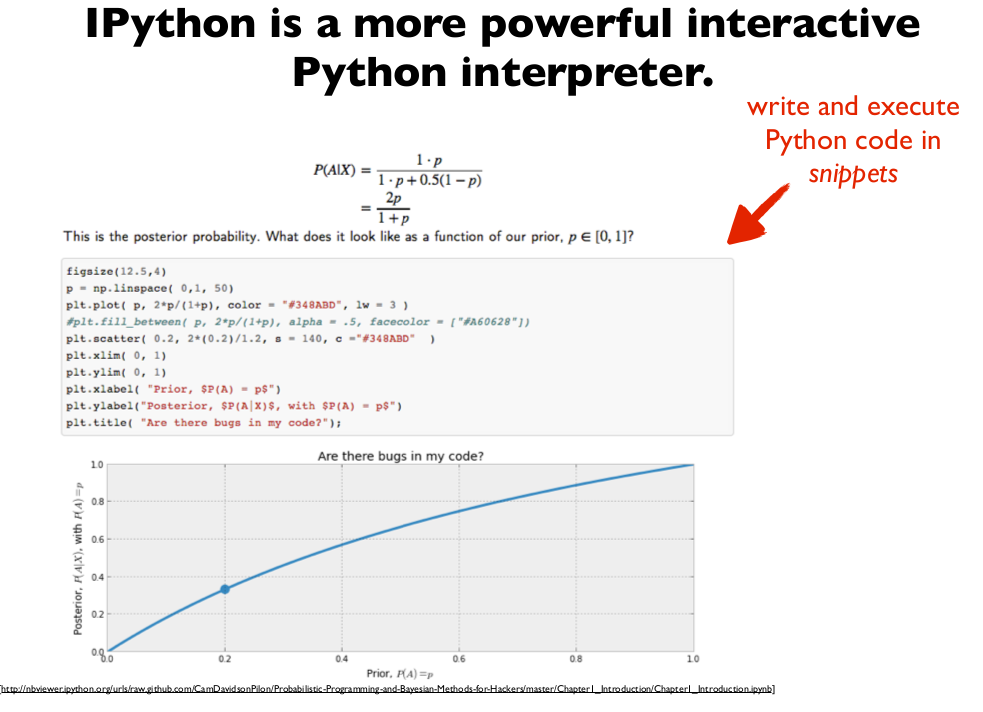
\includegraphics[scale=0.3]{iPythonInterpreter.png}
    \end{center}
\end{frame}
\begin{frame}{}
    \begin{center}
        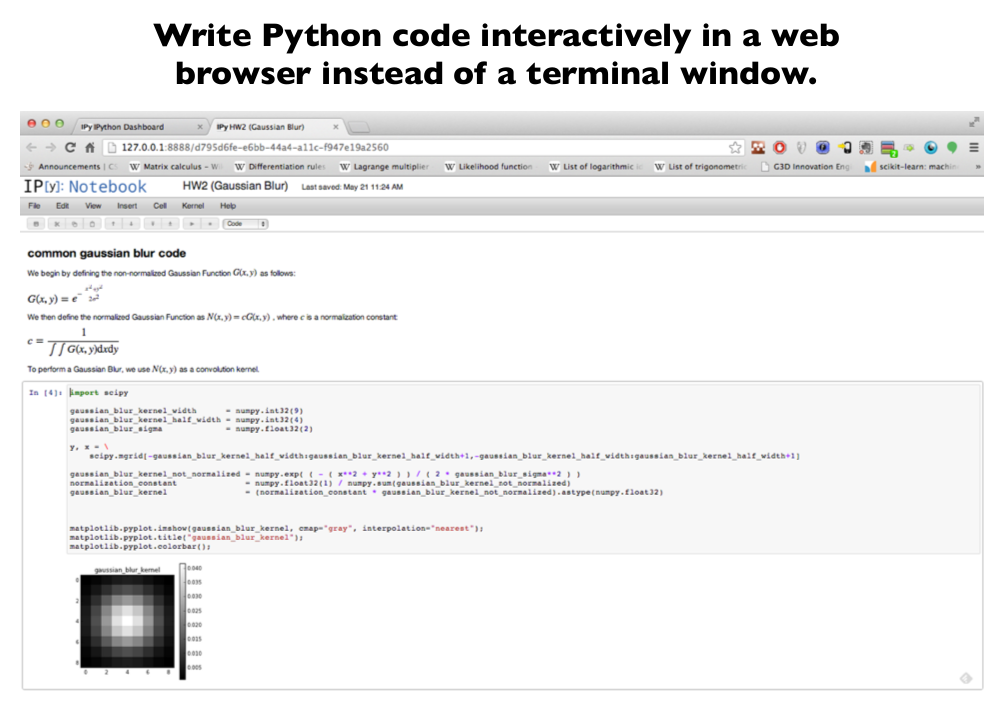
\includegraphics[scale=0.3]{ipythonWeb.png}
    \end{center}
\end{frame}
\begin{frame}{}
    \begin{center}
        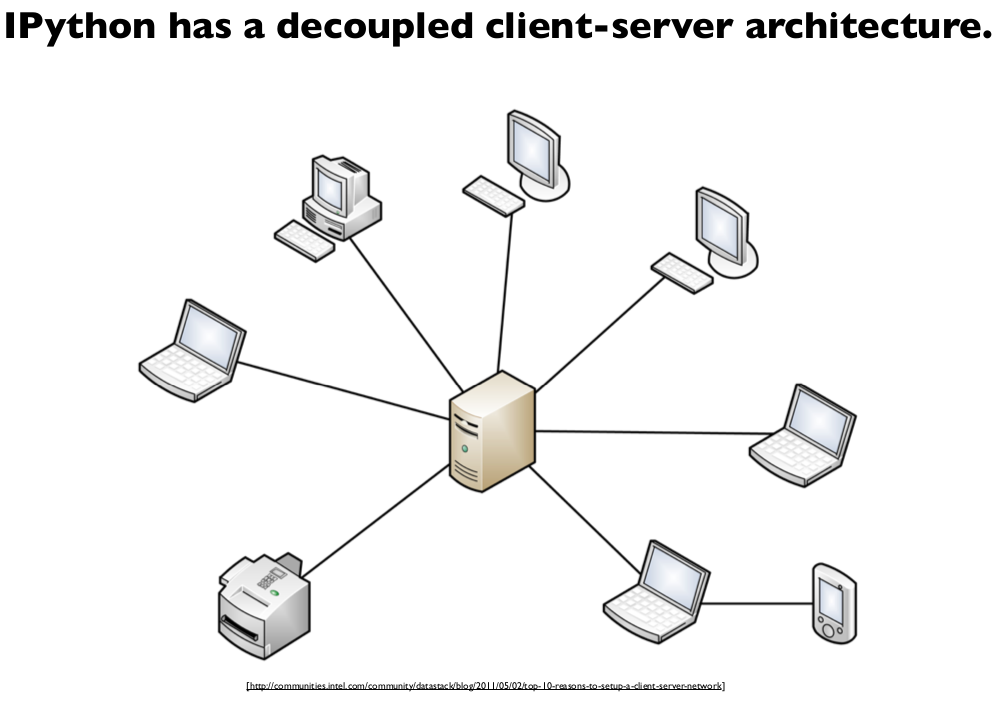
\includegraphics[scale=0.3]{ipythonArch.png}
    \end{center}
\end{frame}
\begin{frame}{}
    \begin{center}
        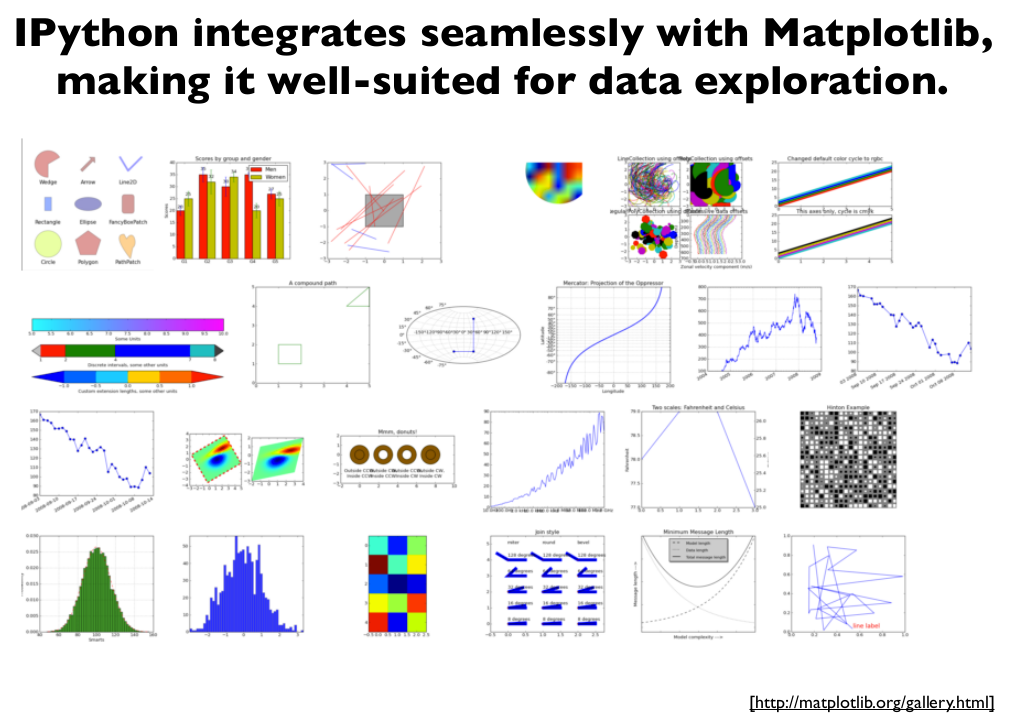
\includegraphics[scale=0.3]{ipythonMatplotlib.png}
    \end{center}
\end{frame}





%\section{Summary}

%\begin{frame}{Summary}

%\tblue{Major Concepts:}
%\begin{itemize}
%\item 
%\end{itemize}
%\end{frame}

\begin{frame}{Slide Material References}

\begin{itemize}
    \item Slides from `Introduction to Statistical Learning' by James, Witten, Hastie, and Tibshirani
    \item Slides from MMDS
    \item Slides from Harvard CS 109 (2013 and 2014)
    \item Slides from Dr.Ryan Tibshirani
\end{itemize}
\end{frame}


\end{document}

